\chapter{Validação}
\label{chap:Chapter6}
O atual capítulo apresenta o processo de validação do modelo proposto, levando em consideração o protótipo desenvolvido. O objetivo é explicar em que se debruçou este processo, demonstrando os resultados obtidos. Primeiramente, foca-se na capacidade do protótipo compreender a linguagem natural, a nível adimensional (sem entidades), unidimensional (com uma entidade) e multidimensional (com várias entidades), ou seja, tenta-se averiguar a avaliação correta das intenções e entidades das questões. De seguida, avalia-se a resposta às questões-chave, procurando-se evidências na competência da extração da informação que se pretende pesquisar com a linguagem natural.

%%%%%%%%%%%%%%%%%%%%%%%%%%%%%%%%%
%           SECTION
%%%%%%%%%%%%%%%%%%%%%%%%%%%%%%%%%
\section{Compreensão da Linguagem Natural}
\label{sec:chap06_comprehension}
O correto funcionamento do \textit{Proto} depende, antes de tudo, da compreensão da linguagem natural e consequentemente, da extração dos conceitos ligados à pergunta colocada. Por isso, usaram-se as perguntas definidas no âmbito dos critérios de sucesso, e apresentadas na Tabela~\ref{tab:proto_intents}, no processo de validação. Na Figura~\ref{fig:nlcomprehesion} mostram-se algumas evidências da análise de perguntas e respetiva extração de intenção e entidades.
%
\begin{figure}
\centering
    \begin{subfigure}[t]{.48\textwidth}
        \centering
        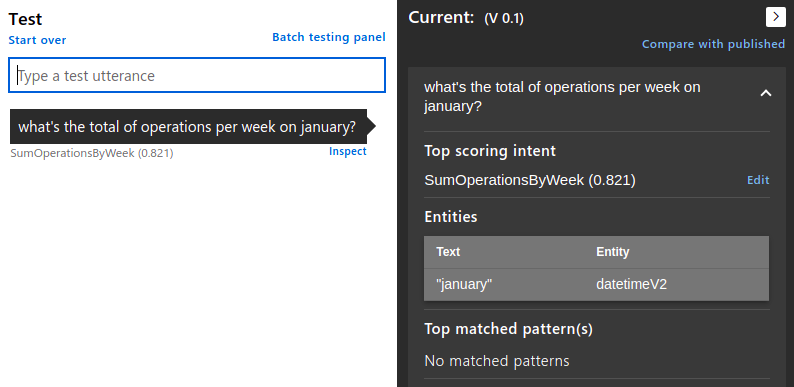
\includegraphics[width=\textwidth]{ch06/assets/nlcomprehension01.png}
        \caption{Intenção \textit{SumOperationsByWeek}}
     \end{subfigure}
     \begin{subfigure}[t]{.48\textwidth}
         \centering
        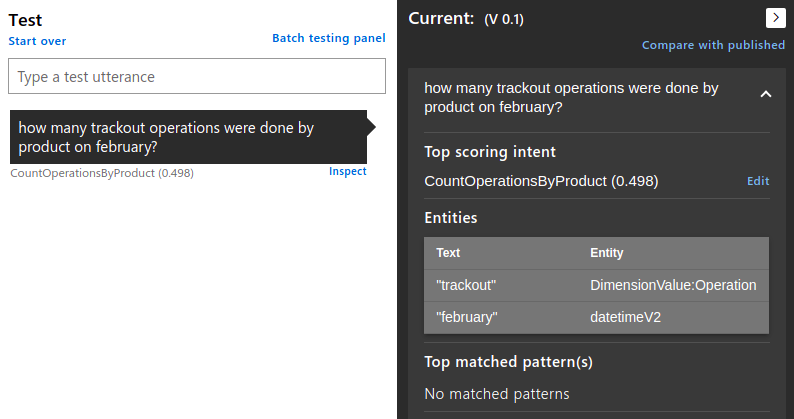
\includegraphics[width=\textwidth]{ch06/assets/nlcomprehension02.png}
        \caption{Intenção \textit{CountOperationByProduct}}
     \end{subfigure}
     \bigbreak
     \begin{subfigure}[t]{.48\textwidth}
        \centering
        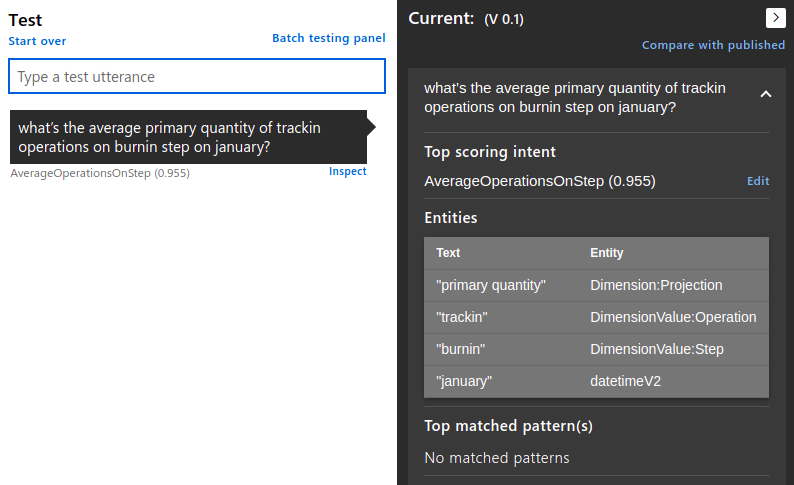
\includegraphics[width=\textwidth]{ch06/assets/nlcomprehension03.png}
        \caption{Intenção \textit{AverageOperationsOnStep}}
     \end{subfigure}
     \begin{subfigure}[t]{.48\textwidth}
        \centering
        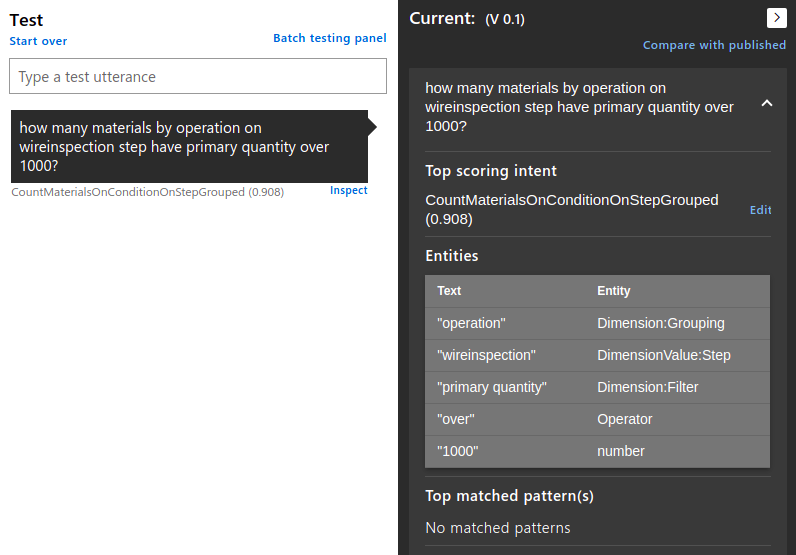
\includegraphics[width=\textwidth]{ch06/assets/nlcomprehension04.png}
        \caption{Intenção \textit{CountOperationsOnConditionOnStepGrouped}}
     \end{subfigure}
\caption{Imagens referentes à avaliação de intenções e entidades do protótipo}
\label{fig:nlcomprehesion}
\end{figure}

O processo de validação consistiu na submissão das perguntas no portal do Microsoft LUIS, o qual possui uma funcionalidade que permite testar o modelo \gls{ml} configurado. A submissão de uma pergunta resulta numa \inquotes{inspeção} completa, discriminando a intenção, classificação resultante, e quais as entidades encontradas na expressão.

Efetivamente, os testes realizados demonstram que protótipo foi capaz de avaliar as perguntas colocadas face à intenção e entidades esperadas visto que, das dez questões avaliadas, ele conseguiu classificá-las de acordo com os critérios. Por outras palavras, valida-se o que protótipo identifica a linguagem natural adimensional, unidimensional e multidimensional.

%%%%%%%%%%%%%%%%%%%%%%%%%%%%%%%%%
%           SECTION
%%%%%%%%%%%%%%%%%%%%%%%%%%%%%%%%%
\section{Resposta às Questões-Chave}
\label{sec:chap06_answers}
Nesta fase da validação, o intuito é avaliar a transformação da representação intermediária e consequente extração da informação. Para esta validação, considerou-se parte do conjunto de dados fornecido pelo supervisor do projeto, que é usado pelo protótipo como fonte de dados. Computaram-se os resultados esperados manualmente, usando uma folha de cálculo, de forma a poder compará-los com a resposta obtida (ver Figura~\ref{fig:nlexpectedanswers}). Posto isto, os cenários considerados para validação são apresentados em seguida:
\begin{enumerate}
    \item
    {
         Nível de linguagem adimensional -- usa-se a questão \textit{What’s the total of operations per week?};
    }
    \item
    {
        Nível de linguagem unidimensional -- a questão considerada é \textit{How many trackout operations were done by product?};
    }
    \item
    {
        Nível de linguagem multidimensional -- corresponde à questão \textit{How many trackout operations were executed by product on February, per shift?}.
    }
\end{enumerate}

\begin{figure}
\centering
    \begin{subfigure}{.55\textwidth}
        \centering
        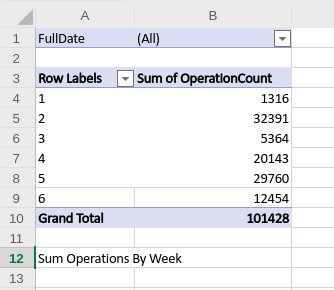
\includegraphics[width=\textwidth]{ch06/assets/expected01.png}
        \caption{Primeiro critério}
     \end{subfigure}
     \begin{subfigure}{.55\textwidth}
         \centering
        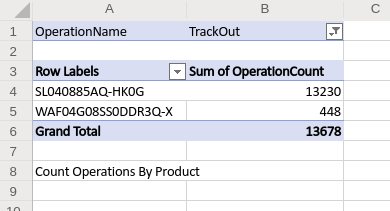
\includegraphics[width=\textwidth]{ch06/assets/expected02.png}
        \caption{Segundo critério}
     \end{subfigure}
     \begin{subfigure}{.55\textwidth}
        \centering
        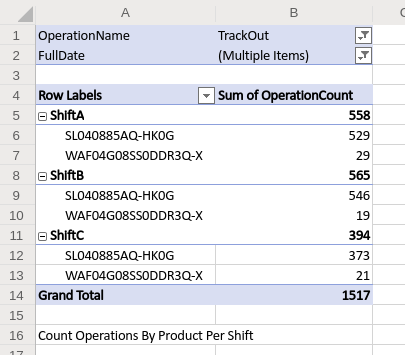
\includegraphics[width=\textwidth]{ch06/assets/expected03.png}
        \caption{Terceiro critério}
     \end{subfigure}
\caption{Imagens referentes aos resultados esperados pelo protótipo, dadas as diferentes perguntas}
\label{fig:nlexpectedanswers}
\end{figure}

Na Figura~\ref{fig:nlanswers} apresentam-se as respostas apresentadas pelo protótipo, no contexto dos critérios apresentados. Adicionalmente, demonstra-se também a forma como o protótipo \inquotes{reage} quando não não possui a resposta que o utilizador espera (ver Figura~\ref{fig:nlanswers_noanswer}). Como se pode observar, a solução consegue dar resposta às perguntas colocadas, estando de acordo com as respostas esperadas.

\begin{figure}
\centering
    \begin{subfigure}[t]{.48\textwidth}
        \centering
        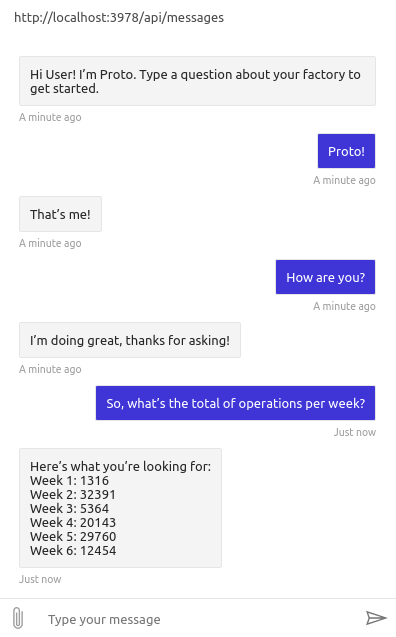
\includegraphics[width=.85\textwidth]{ch06/assets/response01.png}
        \caption{Primeiro critério}
     \end{subfigure}
     \begin{subfigure}[t]{.48\textwidth}
         \centering
        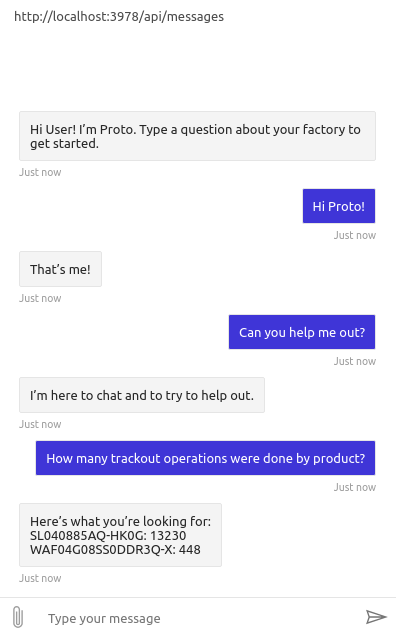
\includegraphics[width=.85\textwidth]{ch06/assets/response02.png}
        \caption{Segundo critério}
     \end{subfigure}
     \bigbreak
     \begin{subfigure}[t]{.48\textwidth}
        \centering
        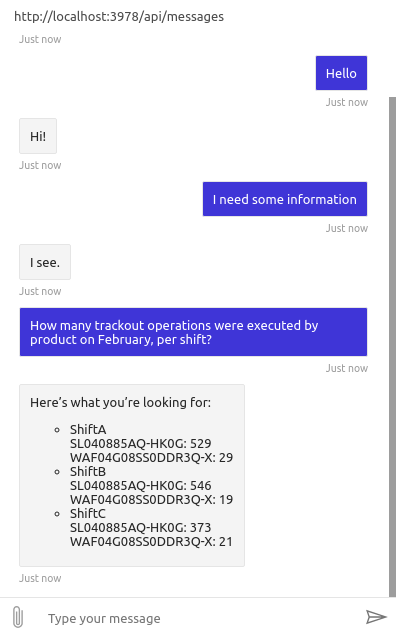
\includegraphics[width=.85\textwidth]{ch06/assets/response03.png}
        \caption{Terceiro critério}
     \end{subfigure}
         \begin{subfigure}[t]{.48\textwidth}
        \centering
        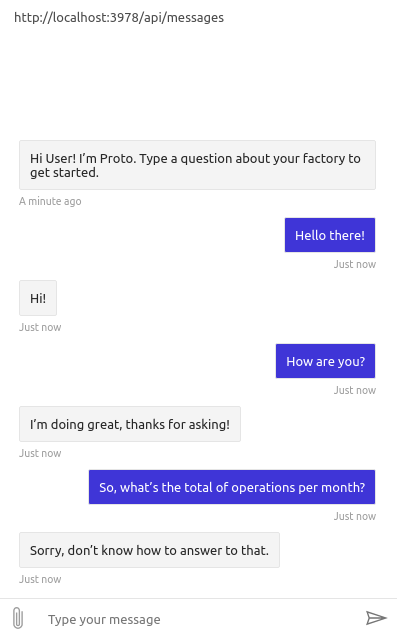
\includegraphics[width=.85\textwidth]{ch06/assets/response04.png}
        \caption{Comportamento do protótipo em caso de não conter a intenção esperada}
        \label{fig:nlanswers_noanswer}
     \end{subfigure}
\caption{Imagens referentes às respostas dadas pelo protótipo, dadas diferentes perguntas}
\label{fig:nlanswers}
\end{figure}

% para os quais se usou o ficheiro de dados fornecido pelo supervisor do projeto, usado pelo protótipo na simulação da base de dados relacional. Para a avaliação de cada cenário, computou-se o(s) resultado(s) esperados manualmente, usando uma folha de cálculo. Posto isto, os cenários considerados para validação são:
% %
% \begin{enumerate}
%     \item
%     {
%         Interação com o \textit{Proto} com conversa casual e fazer a pergunta \textit{What’s the total of operations per week on February?} -- o \textit{Proto} deve ser capaz de responder fluentemente, indicando que a resposta a esta última questão é de $11942$ operações na semana $6$;
%     }
%     \item 
%     {
%         Fazer a pergunta \textit{How many trackout operations were executed by product on January?} e agradecer -- espera-se que o \textit{Proto} responda que foram executadas $11782$ e $379$ operações para os produtos SL040885AQ-HK0G e WAF04G08SS0DDR3Q-X, respetivamente;
%     }
%     \item
%     {
%         Perguntar \textit{What’s the average primary quantity of trackin operations on burninstep on March?} -- neste caso, visto não existir dados referentes a Março no conjunto de dados, o \textit{Probot} deve \inquotes{falhar} graciosamente, dizendo que não consegue
%     }
% \end{enumerate}

%%%%%%%%%%%%%%%%%%%%%%%%%%%%%%%%%
%           SECTION
%%%%%%%%%%%%%%%%%%%%%%%%%%%%%%%%%
\section{Síntese}
\label{sec:chap06_chaptersummary}
Este capítulo abordou o processo de validação do protótipo desenvolvido, tendo em conta dois requisitos: a compreensão da linguagem natural nos vários níveis considerados e a resposta às questões-chave apresentadas no capítulo anterior.

Para a primeira verificou-se que a solução é capaz de lidar com a linguagem natural, extraindo as intenções e entidades que são esperadas. 

No caso da segunda, demonstrou-se que o protótipo responde a questões-chave, e também que é capaz de responder adequadamente em caso de não conter a resposta procurada pelo utilizador.